\Transcb{yellow}{blue}{Coordinate systems}
\onecolumn
\begin{itemize}
\item Celestial positions : Convenient to use spherical coordinates $(r,\theta,\phi)$
\item[] In indicating a direction, the distance doesn't matter $\rightarrow$ Ignore $r$
\item Celestial positions are indicated by two angles called {\blue latitude} and {\blue longitude}
\item[] But w.r.t. to which origin are these angles provided ?
\item[$\ast$] Define an {\blue equator} by taking a so called {\blue great circle}
\item[] Great circle : Centered at the sphere center and encompasses the full sphere
\item \colorbox{yellow}{The equator indicates the zero of latitude}
\item[$\ast$] {\blue Choose a location on the equator as zero for the longitude}
\item[] Define the directions of positive and negative latitude and longitude
\item[] The lines of constant longitude are called {\blue meridians}
\item Reference systems like this are called {\blue celestial reference systems}
\item[] It is obvious that there are many different possibilities for such a system 
\end{itemize}

\Tr
\onecolumn
\begin{center}
{\blue A generic celestial reference system}\\[3mm]
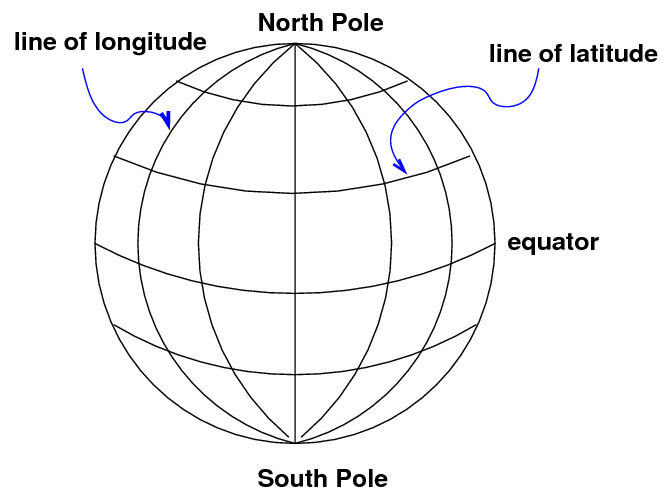
\includegraphics[keepaspectratio,height=14cm]{gen-ref}
\end{center}

\Tr
\onecolumn
\begin{center}
{\red Horizon coordinates}
\end{center}
%
\begin{itemize}
\item Imagine standing at night in an open field without any houses, trees etc.
\item[] You feel as if you are the centre of everything
\item \colorbox{yellow}{Conventions to define the observer centered reference system}
\item[] The point straight above is called {\blue Zenith} and straight below is called {\blue Nadir}
\item[$\ast$] \colorbox{yellow}{Take the horizon as equator}
\item[] The (latitude) {\blue angle above the horizon} of a star's position is called {\blue Altitude}
\item[] Alternatively the angle w.r.t. the Zenith ({\blue Zenith angle}) of a star can be given
\item[$\ast$] \colorbox{yellow}{Take the North point on the equator as zero longitude}
\item[] The (longitude) {\blue angle measured eastwards} to a star's position is called {\blue Azimuth}
\item[$\ast$] Notes :
\item[] \colorbox{yellow}{For an observer at a Pole, Greenwich defines the zero longitude}
\item[] Values of altitude and azimuth depend on the location of the observer
\item[] Values of altitude and azimuth change fast due to the Earth's spin
\end{itemize}

\Tr
\onecolumn
\begin{center}
{\blue The horizon coordinate system}\\[3mm]
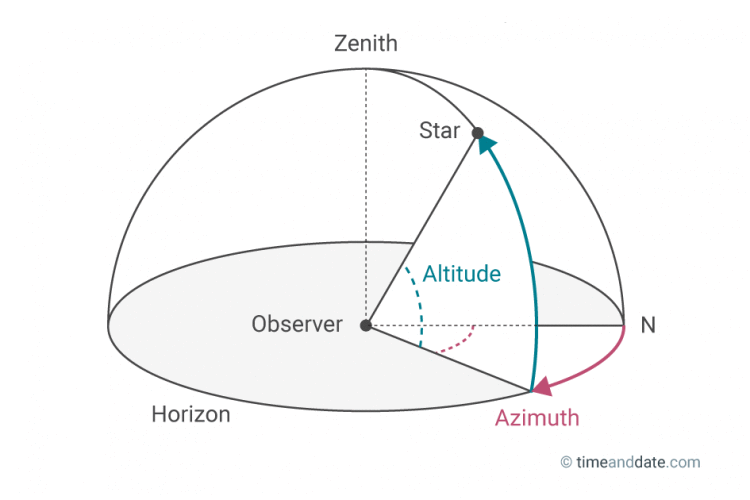
\includegraphics[keepaspectratio,height=14cm]{alt-azi}
\end{center}

\Tr
\onecolumn
\begin{center}
{\red Equatorial coordinates}
\end{center}
%
\begin{itemize}
\item Imagine standing on one of the Poles at the Earth's spin axis
\item[] With time the azimuth of a star will change, but not its altitude
\item[] This is quite convenient if one wants to follow a certain object
\item[$\ast$] Due to the coincidence of the Zenith-Nadir axis with the Earth's spin axis
\item[] $\rightarrow$ Your equator coincides with the Earth's equator
\item \colorbox{yellow}{Conventions to define the equatorial celestial reference system}
\item[$\ast$] {\blue Take the center of the Earth as the center of the reference system}
\item[$\ast$] \colorbox{yellow}{Take the (projection of) the Earth equator as equator}
\item[] This projection is called the {\blue celestial equator}
\item[] The {\blue angle above the equator} of a star's position is called {\blue Declination}
\item[] The angle of longitude is called {\blue Right Ascension}
\item {\red What to take as zero longitude ?}
\item[] Preferably a point that doesn't change with time.
\end{itemize}

\Tr
\onecolumn
\begin{center}
{\blue The equatorial celestial reference system}\\[3mm]
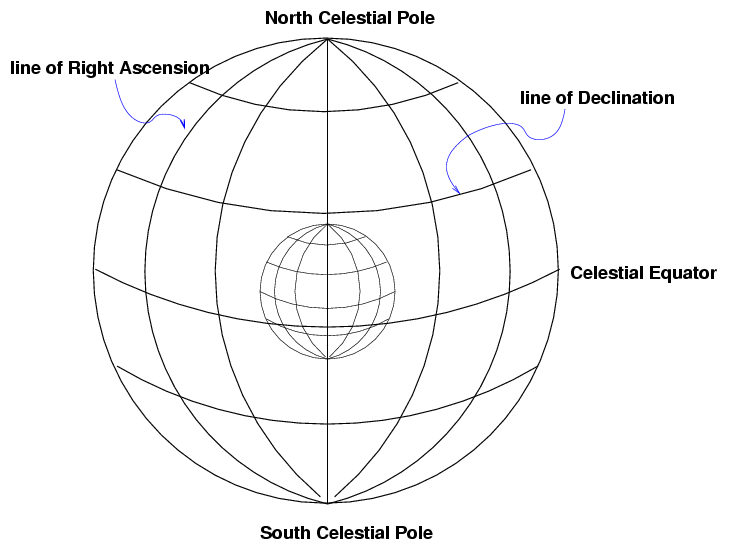
\includegraphics[keepaspectratio,height=14cm]{equatorial-ref}
\end{center}

\Tr
\onecolumn
\begin{itemize}
\item The Earth rotates around the Sun in a fixed plane
\item[] The Earth's spin axis is inclined ($\sim 23.4^{\circ}$) with the normal to this plane
\item Imagine that the Earth only rotates around the Sun; no spin around its axis
\item[] Consider the Earth as a perfect sphere
\item[] Observe from the Earth's center the position of the Sun over the year 
\item[] Project the Sun's trajectory on the Earth's surface
\item[] $\rightarrow$ This projection is a great circle inclined ($\sim 23.4^{\circ}$) with the equator
\item[] This projection of the Sun's trajectory is called the {\blue ecliptic}
\item The ecliptic will cross the equator twice per year
\item[] Going from South to North in spring $\rightarrow$ {\blue Vernal equinox}
\item[] Going from North to South in autumn $\rightarrow$ {\blue Autumn equinox}
\item[$\ast$] \colorbox{yellow}{Take the Vernal equinox on the equator as zero longitude}
\item[] The {\blue angle measured eastwards} to a star's position is called {\blue Right Ascension}
\end{itemize}

\Tr
\onecolumn
\begin{center}
{\blue The equatorial coordinate system}\\[3mm]
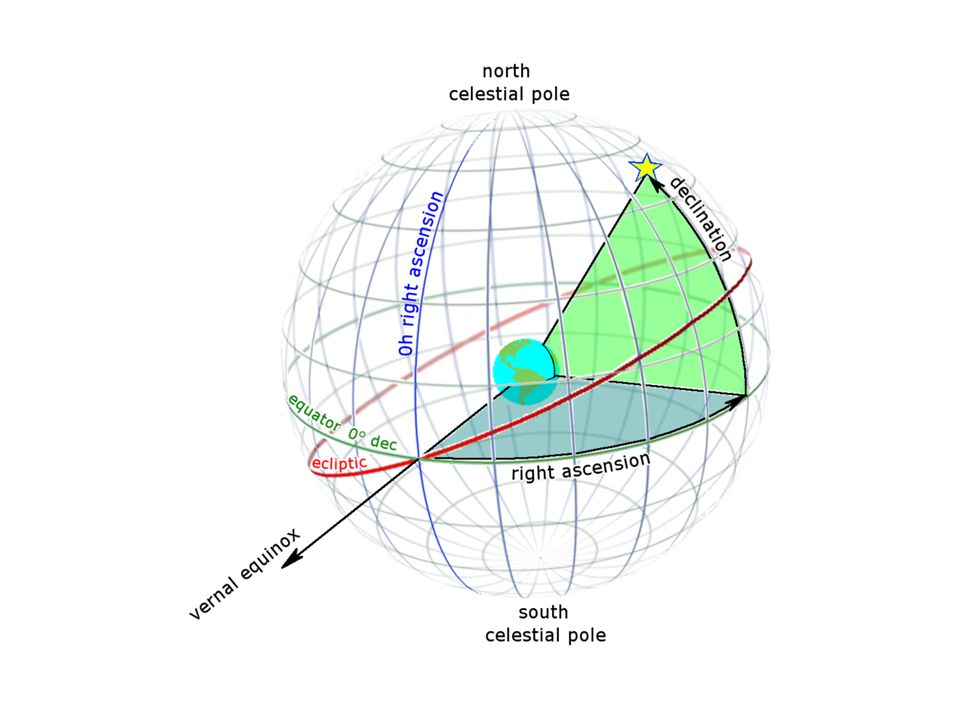
\includegraphics[keepaspectratio,height=14cm]{ra-dec}
\end{center}

\Tr
\onecolumn
\begin{itemize}
\item Precession of the Earth's spin axis $\rightarrow$ Vernal equinox shifts along the equator
\item[] One full turn ($360^{\circ}$) in 25770 years $\rightarrow$ Quite a stable point
\item[] Once every 50 years (epoch) the Vernal equinox position is updated
\item The nutation of the Earth's spin axis induces also (minor) shifts in declinations
\end{itemize}
%
\begin{center}
{\red Notation conventions}
\end{center}
%
\begin{itemize}
\item {\blue Declination ($\delta$)} is indicated in degrees (North +, South --)
\item {\blue Right Ascension ($\alpha$)} is indicated in hours, minutes, seconds
\item[] 1 Full revolution ($360^{\circ}$) in 24 hours $\rightarrow$ 1 hour = $15^{\circ}$
\item The average epoch coordinates we call {\blue Mean coordinates}
\item[] The Mean $(\alpha,\delta)$ contain the precession correction, but not the nutation
\item Including also the nutation correction we speak of {\blue True coordinates}
\item[$\ast$] So it is important to denote w.r.t. to which epoch origin the $(\alpha,\delta)$ are given
\item[] Nowadays we use the update at the start of the year 2000 (i.e. J2000)
\end{itemize}

\Tr
\onecolumn
\begin{center}
{\blue Equatorial coordinate notations}\\[3mm]
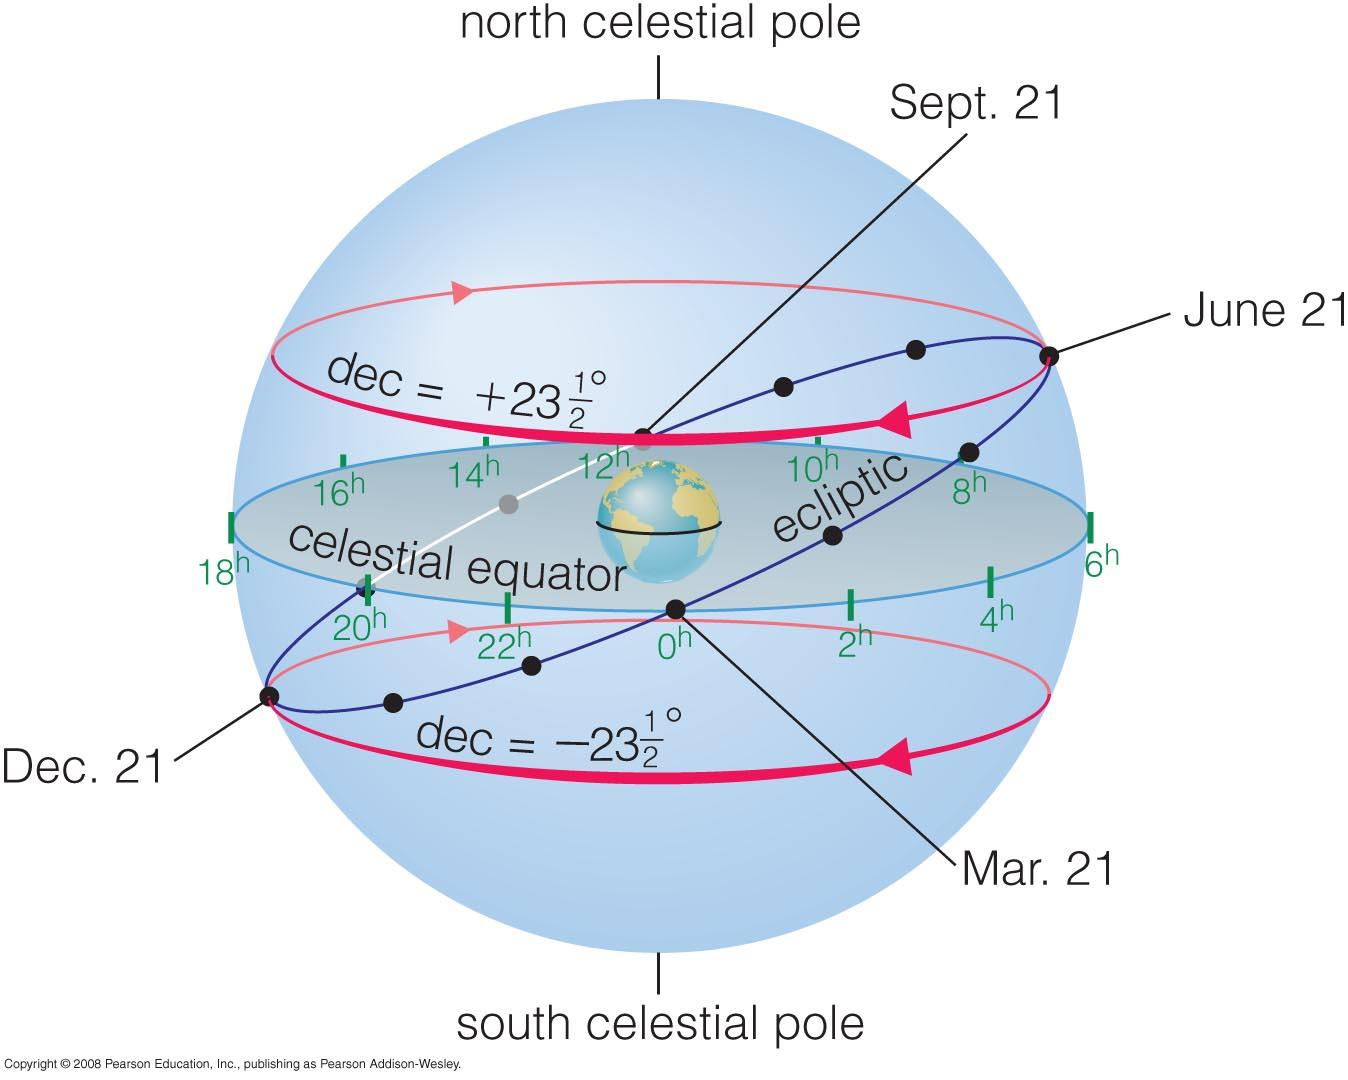
\includegraphics[keepaspectratio,height=14cm]{hra-dec}
\end{center}

\Tr
\onecolumn
%
\begin{center}
{\red Indicating directions in the Universe}
\end{center}
%
\begin{itemize}
\item We have seen that $(\alpha,\delta)$ provide rather constant coordinates
\item[] Use these to indicate a certain direction in the Universe
\item Convert track directions $(\theta,\phi)$ in IceCube to $(\alpha,\delta)$
\item[] $\rightarrow$ Enables us to look for cosmic neutrino sources
\end{itemize}
%
\begin{center}
{\red Sidereal Time}
\end{center}
%
\begin{itemize}
\item As the Earth spins around its axis, different stars will cross a certain meridian
\item[$\ast$] \colorbox{yellow}{Sidereal Time $\equiv \alpha$ of the stars that cross the observer's meridian}
\item Since we can use the {\blue Mean and True coordinates} we define
\item[] {\red LMST : Local Mean Sidereal Time}
\item[] {\red LAST : Local Apparent Sidereal Time}
\item[] {\red GMST : Greenwich Mean Sidereal Time}
\item[] {\red GAST : Greenwich Apparent Sidereal Time}
\end{itemize}
